\documentclass{standalone}
\usepackage{tikz}
\usetikzlibrary{patterns}
\usetikzlibrary{positioning}
\usetikzlibrary{patterns, positioning}
\usetikzlibrary{shapes.misc}
\usepackage[outline]{contour}
\contourlength{1.5pt} 
\usepackage[sfdefault]{ClearSans}

\begin{document}
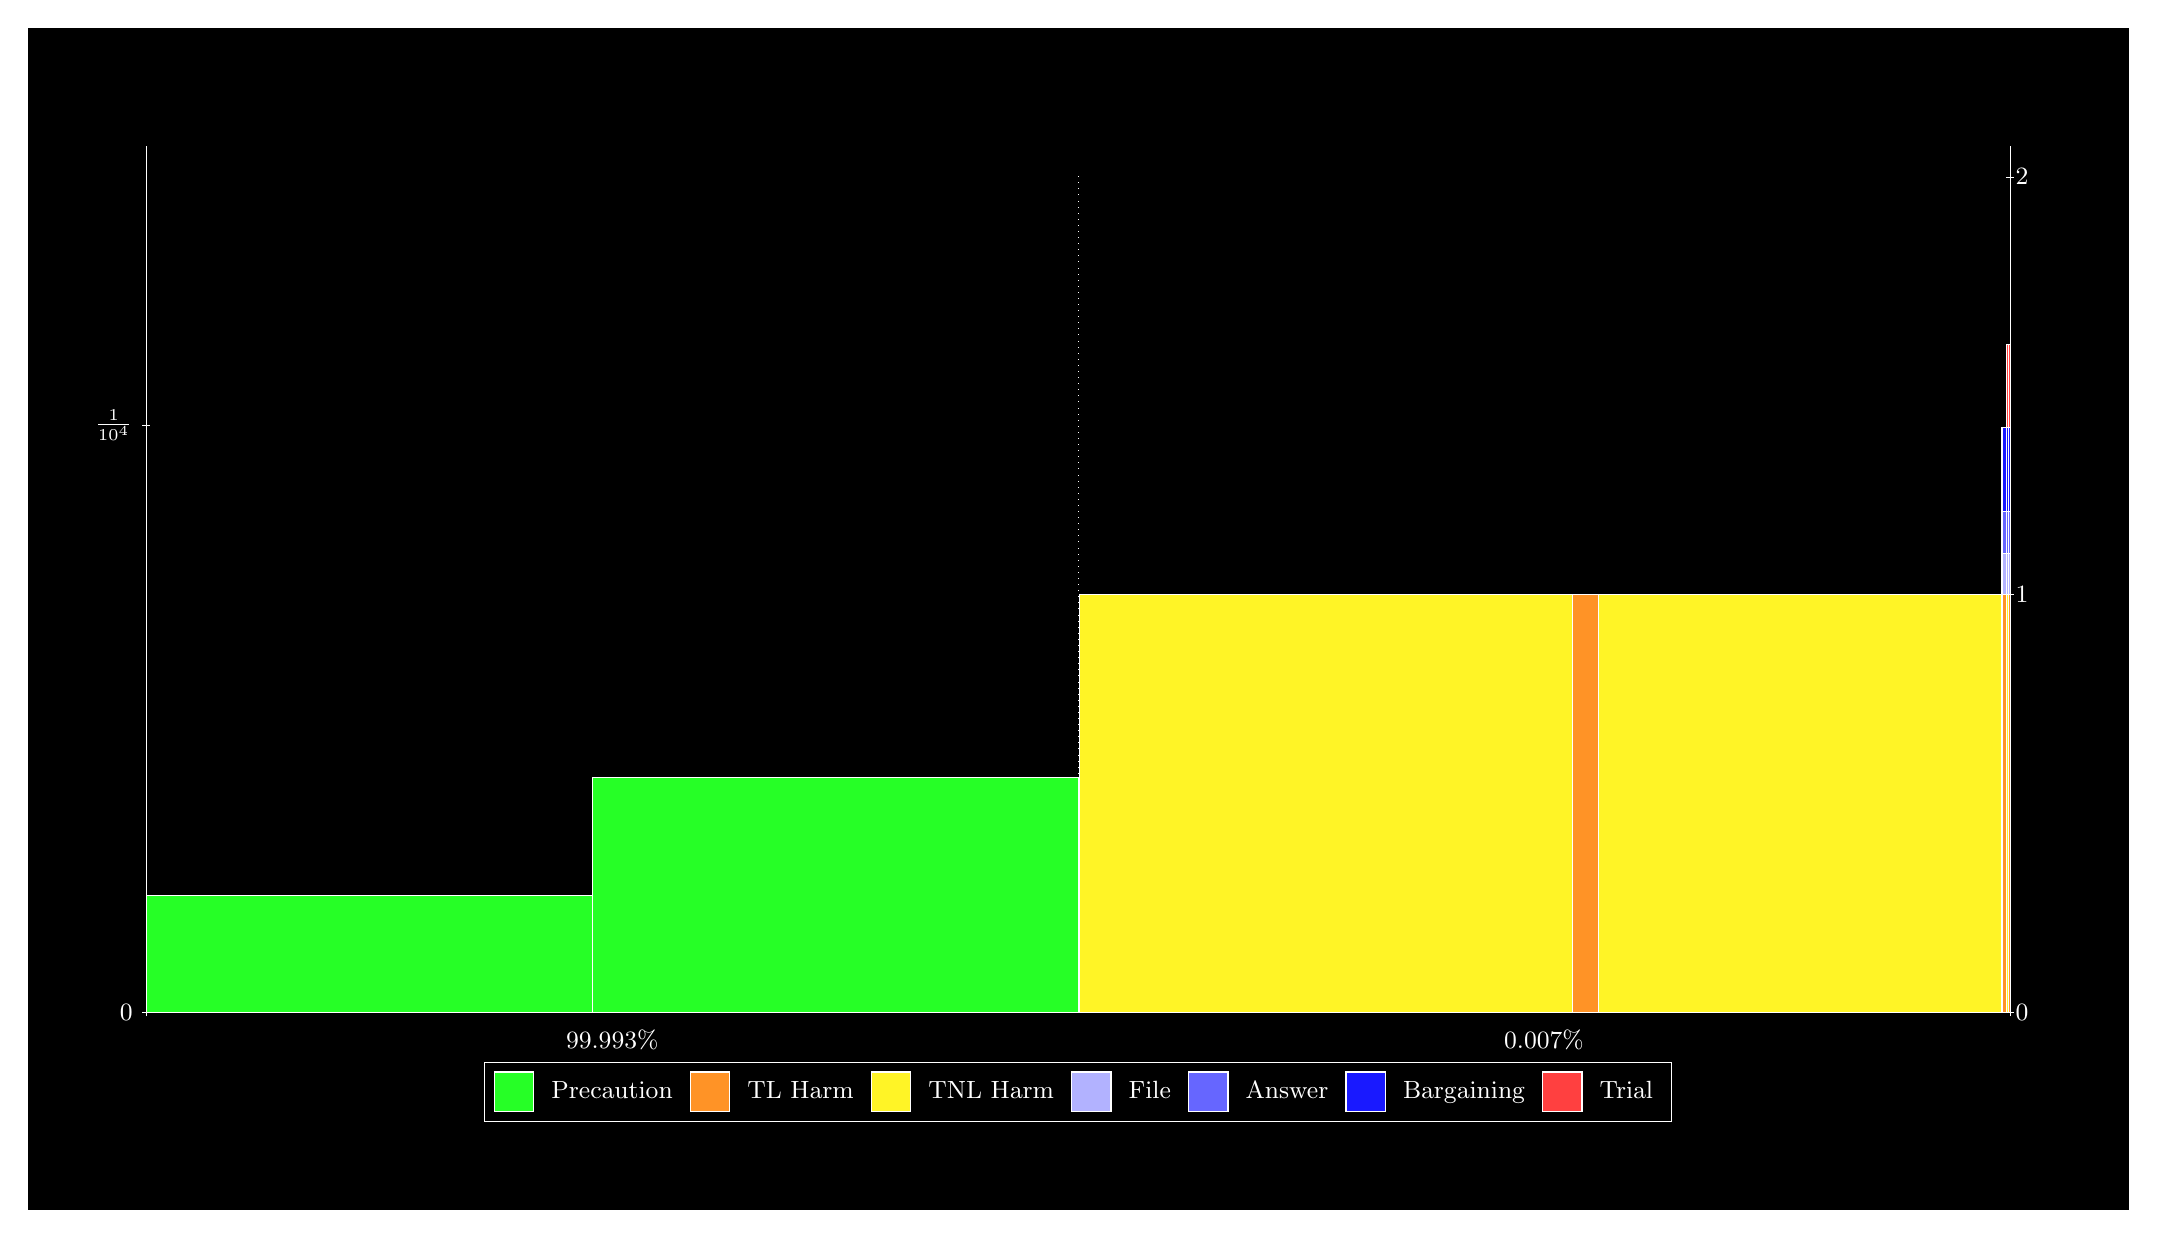
\begin{tikzpicture}
\draw[fill=black] (0,0) rectangle (26.667,15);
\draw[fill=green!85,draw=white,very thin] (1.5,2.5) rectangle (7.1597,3.9918);
\draw[fill=green!85,draw=white,very thin] (7.1597,2.5) rectangle (13.333,5.4837);
\draw[fill=green!85,draw=white,very thin] (13.333,2.5) rectangle (13.342,2.5001);
\draw[fill=blue!30,draw=white,very thin] (13.333,2.5001) rectangle (13.342,3.0307);
\draw[fill=blue!60,draw=white,very thin] (13.333,3.0307) rectangle (13.342,3.5614);
\draw[fill=blue!90,draw=white,very thin] (13.333,3.5614) rectangle (13.342,4.6226);
\draw[fill=green!85,draw=white,very thin] (13.342,2.5) rectangle (13.347,2.5001);
\draw[fill=blue!30,draw=white,very thin] (13.342,2.5001) rectangle (13.347,3.0307);
\draw[fill=blue!60,draw=white,very thin] (13.342,3.0307) rectangle (13.347,3.5614);
\draw[fill=blue!90,draw=white,very thin] (13.342,3.5614) rectangle (13.347,4.6226);
\draw[fill=red!75,draw=white,very thin] (13.342,4.6226) rectangle (13.347,5.6839);
\draw[fill=green!85,draw=white,very thin] (13.347,2.5) rectangle (19.611,2.5001);
\draw[fill=yellow!85,draw=white,very thin] (13.347,2.5001) rectangle (19.611,7.8065);
\draw[fill=green!85,draw=white,very thin] (19.611,2.5) rectangle (19.938,2.5001);
\draw[fill=orange!85,draw=white,very thin] (19.611,2.5001) rectangle (19.938,7.8065);
\draw[fill=green!85,draw=white,very thin] (19.938,2.5) rectangle (25.056,2.5002);
\draw[fill=yellow!85,draw=white,very thin] (19.938,2.5002) rectangle (25.056,7.8066);
\draw[fill=green!85,draw=white,very thin] (25.056,2.5) rectangle (25.074,2.5001);
\draw[fill=yellow!85,draw=white,very thin] (25.056,2.5001) rectangle (25.074,7.8065);
\draw[fill=blue!30,draw=white,very thin] (25.056,7.8065) rectangle (25.074,8.3371);
\draw[fill=blue!60,draw=white,very thin] (25.056,8.3371) rectangle (25.074,8.8677);
\draw[fill=blue!90,draw=white,very thin] (25.056,8.8677) rectangle (25.074,9.929);
\draw[fill=green!85,draw=white,very thin] (25.074,2.5) rectangle (25.122,2.5001);
\draw[fill=orange!85,draw=white,very thin] (25.074,2.5001) rectangle (25.122,7.8065);
\draw[fill=blue!30,draw=white,very thin] (25.074,7.8065) rectangle (25.122,8.3371);
\draw[fill=blue!60,draw=white,very thin] (25.074,8.3371) rectangle (25.122,8.8677);
\draw[fill=blue!90,draw=white,very thin] (25.074,8.8677) rectangle (25.122,9.929);
\draw[fill=green!85,draw=white,very thin] (25.122,2.5) rectangle (25.145,2.5001);
\draw[fill=yellow!85,draw=white,very thin] (25.122,2.5001) rectangle (25.145,7.8065);
\draw[fill=blue!30,draw=white,very thin] (25.122,7.8065) rectangle (25.145,8.3371);
\draw[fill=blue!60,draw=white,very thin] (25.122,8.3371) rectangle (25.145,8.8677);
\draw[fill=blue!90,draw=white,very thin] (25.122,8.8677) rectangle (25.145,9.929);
\draw[fill=red!75,draw=white,very thin] (25.122,9.929) rectangle (25.145,10.99);
\draw[fill=green!85,draw=white,very thin] (25.145,2.5) rectangle (25.167,2.5001);
\draw[fill=orange!85,draw=white,very thin] (25.145,2.5001) rectangle (25.167,7.8065);
\draw[fill=blue!30,draw=white,very thin] (25.145,7.8065) rectangle (25.167,8.3371);
\draw[fill=blue!60,draw=white,very thin] (25.145,8.3371) rectangle (25.167,8.8677);
\draw[fill=blue!90,draw=white,very thin] (25.145,8.8677) rectangle (25.167,9.929);
\draw[fill=red!75,draw=white,very thin] (25.145,9.929) rectangle (25.167,10.99);
\draw[white,very thin] (1.5,2.5) -- (1.5,13.5);
\draw[white,very thin] (1.45,2.5) -- (1.55,2.5);
\node[font=\small,text=white, anchor=east] at (1.45, 2.5) {0};
\draw[white,very thin] (1.45,9.9592) -- (1.55,9.9592);
\node[font=\small,text=white, anchor=east] at (1.45, 9.9592) {$\frac{1}{10^{4}}$};

\draw[white,dotted,very thin] (13.333,2.83) -- (13.333,13.17);
\draw[white,very thin] (25.167,2.5) -- (25.167,13.5);
\draw[white,very thin] (25.117,2.5) -- (25.217,2.5);
\node[font=\small,text=white, anchor=west] at (25.117, 2.5) {0};
\draw[white,very thin] (25.117,7.8064) -- (25.217,7.8064);
\node[font=\small,text=white, anchor=west] at (25.117, 7.8064) {1};
\draw[white,very thin] (25.117,13.113) -- (25.217,13.113);
\node[font=\small,text=white, anchor=west] at (25.117, 13.113) {2};

\draw[white,very thin] (1.5,2.5) -- (25.167,2.5);
\draw[white,very thin] (1.5,2.45) -- (1.5,2.55);
\node[font=\small,text=white, anchor=north] at (1.5, 2.45) {};
\draw[white,very thin] (25.167,2.45) -- (25.167,2.55);
\node[font=\small,text=white, anchor=north] at (25.167, 2.45) {};

\node[font=\small,text=white,anchor=south] at (7.4167, 1.9) {99.993\%};
\node[font=\small,text=white,anchor=south] at (19.25, 1.9) {0.007\%};
\draw (13.3333,2.5) node (B) {};
\begin{scope}[align=center]
\matrix[scale=0.5,draw=white,below=0.5cm of B,nodes={draw},column sep=0.1cm]{
\node[rectangle,draw,minimum width=0.5cm,minimum height=0.5cm,fill=green!85]{}; & \node[draw=none,font=\small,text=white]{Precaution}; &
\node[rectangle,draw,minimum width=0.5cm,minimum height=0.5cm,fill=orange!85]{}; & \node[draw=none,font=\small,text=white]{TL Harm}; &
\node[rectangle,draw,minimum width=0.5cm,minimum height=0.5cm,fill=yellow!85]{}; & \node[draw=none,font=\small,text=white]{TNL Harm}; &
\node[rectangle,draw,minimum width=0.5cm,minimum height=0.5cm,fill=blue!30]{}; & \node[draw=none,font=\small,text=white]{File}; &
\node[rectangle,draw,minimum width=0.5cm,minimum height=0.5cm,fill=blue!60]{}; & \node[draw=none,font=\small,text=white]{Answer}; &
\node[rectangle,draw,minimum width=0.5cm,minimum height=0.5cm,fill=blue!90]{}; & \node[draw=none,font=\small,text=white]{Bargaining}; &
\node[rectangle,draw,minimum width=0.5cm,minimum height=0.5cm,fill=red!75]{}; & \node[draw=none,font=\small,text=white]{Trial}; \\\\
};\end{scope}

\end{tikzpicture}
\end{document}